\section{Date: 2026-11-26}
\noindent \textbf{Series ID: NCOTOT38} 

\noindent This series is titled Total Net Loan Charge-offs to Total Loans, Banks with Total Assets from \$1B to \$10B, Mountain Census Division (DISCONTINUED) and has a frequency of Quarterly, End of Period. The units are Percent and the seasonal adjustment is Not Seasonally Adjusted.The observation start date is 1988-01-01 and the observation end date is 2020-07-01.The popularity of this series is 3. \\ 

\noindent \textbf{Series ID: BOPBIIA} 

\noindent This series is titled Balance on Investment Income (DISCONTINUED) and has a frequency of Annual. The units are Billions of Dollars and the seasonal adjustment is Not Seasonally Adjusted.The observation start date is 1960-01-01 and the observation end date is 2013-01-01.The popularity of this series is 1. \\ 

\subsection{Raw Regression}
\noindent Regresses the two series against each other directly. A significant result here can come just as easily from both series sharing a long-run trend as from any real relationship.

\begin{center}
\begin{tabular}{lclc}
\toprule
\textbf{Dep. Variable:}        & value\_fred\_BOPBIIA & \textbf{  R-squared:         } &     0.007   \\
\textbf{Model:}                &         OLS          & \textbf{  Adj. R-squared:    } &    -0.034   \\
\textbf{Method:}               &    Least Squares     & \textbf{  F-statistic:       } &    0.1812   \\
\textbf{Date:}                 &   Thu, 26 Nov 2026   & \textbf{  Prob (F-statistic):} &    0.674    \\
\textbf{Time:}                 &       20:37:49       & \textbf{  Log-Likelihood:    } &   -146.16   \\
\textbf{No. Observations:}     &            26        & \textbf{  AIC:               } &     296.3   \\
\textbf{Df Residuals:}         &            24        & \textbf{  BIC:               } &     298.8   \\
\textbf{Df Model:}             &             1        & \textbf{                     } &             \\
\textbf{Covariance Type:}      &      nonrobust       & \textbf{                     } &             \\
\bottomrule
\end{tabular}
\begin{tabular}{lcccccc}
                               & \textbf{coef} & \textbf{std err} & \textbf{t} & \textbf{P$> |$t$|$} & \textbf{[0.025} & \textbf{0.975]}  \\
\midrule
\textbf{const}                 &      74.5646  &       26.025     &     2.865  &         0.009        &       20.852    &      128.277     \\
\textbf{value\_fred\_NCOTOT38} &      -6.7005  &       15.741     &    -0.426  &         0.674        &      -39.189    &       25.788     \\
\bottomrule
\end{tabular}
\begin{tabular}{lclc}
\textbf{Omnibus:}       &  7.778 & \textbf{  Durbin-Watson:     } &    0.107  \\
\textbf{Prob(Omnibus):} &  0.020 & \textbf{  Jarque-Bera (JB):  } &    7.015  \\
\textbf{Skew:}          &  1.272 & \textbf{  Prob(JB):          } &   0.0300  \\
\textbf{Kurtosis:}      &  3.021 & \textbf{  Cond. No.          } &     4.06  \\
\bottomrule
\end{tabular}
%\caption{OLS Regression Results}
\end{center}

Notes: \newline
 [1] Standard Errors assume that the covariance matrix of the errors is correctly specified.

\begin{figure}
\centering
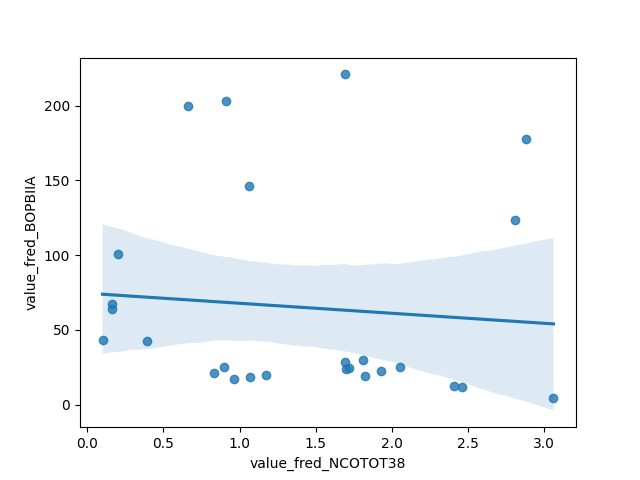
\includegraphics[scale = 0.9]{plots/plot_2026-11-26.png}
\caption{Raw Regression Plot for 2026-11-26}
\end{figure}
\newpage
\subsection{Detrended Regression}
\noindent Regresses the residuals of each series after removing its own linear time trend, so a shared trend can no longer drive the result on its own. A relationship that stays significant here is better evidence of a genuine link between the two series.

\begin{center}
\begin{tabular}{lclc}
\toprule
\textbf{Dep. Variable:}                   & value\_fred\_BOPBIIA\_detrended & \textbf{  R-squared:         } &     0.000   \\
\textbf{Model:}                           &               OLS               & \textbf{  Adj. R-squared:    } &    -0.042   \\
\textbf{Method:}                          &          Least Squares          & \textbf{  F-statistic:       } & 0.0009872   \\
\textbf{Date:}                            &         Thu, 26 Nov 2026        & \textbf{  Prob (F-statistic):} &    0.975    \\
\textbf{Time:}                            &             20:37:49            & \textbf{  Log-Likelihood:    } &   -131.56   \\
\textbf{No. Observations:}                &                  26             & \textbf{  AIC:               } &     267.1   \\
\textbf{Df Residuals:}                    &                  24             & \textbf{  BIC:               } &     269.6   \\
\textbf{Df Model:}                        &                   1             & \textbf{                     } &             \\
\textbf{Covariance Type:}                 &            nonrobust            & \textbf{                     } &             \\
\bottomrule
\end{tabular}
\begin{tabular}{lcccccc}
                                          & \textbf{coef} & \textbf{std err} & \textbf{t} & \textbf{P$> |$t$|$} & \textbf{[0.025} & \textbf{0.975]}  \\
\midrule
\textbf{const}                            &   -2.789e-13  &        7.783     & -3.58e-14  &         1.000        &      -16.063    &       16.063     \\
\textbf{value\_fred\_NCOTOT38\_detrended} &       0.2838  &        9.031     &     0.031  &         0.975        &      -18.356    &       18.923     \\
\bottomrule
\end{tabular}
\begin{tabular}{lclc}
\textbf{Omnibus:}       &  3.767 & \textbf{  Durbin-Watson:     } &    0.309  \\
\textbf{Prob(Omnibus):} &  0.152 & \textbf{  Jarque-Bera (JB):  } &    1.580  \\
\textbf{Skew:}          &  0.185 & \textbf{  Prob(JB):          } &    0.454  \\
\textbf{Kurtosis:}      &  1.850 & \textbf{  Cond. No.          } &     1.16  \\
\bottomrule
\end{tabular}
%\caption{OLS Regression Results}
\end{center}

Notes: \newline
 [1] Standard Errors assume that the covariance matrix of the errors is correctly specified.

\begin{figure}
\centering
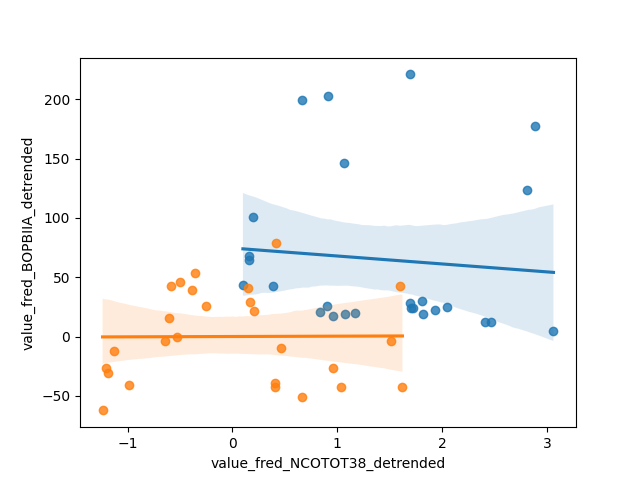
\includegraphics[scale = 0.9]{plots/plot_2026-11-26_detrended.png}
\caption{Detrended Regression Plot for 2026-11-26}
\end{figure}
\newpage
